\documentclass[main.tex]{subfiles}

\begin{document}

\subsection{Secondo esercizio}

\begin{figure}[H]
\centering
\includegraphics[width=0.75\textwidth]{2017-1109-2.jpg}
\end{figure}

Il sistema rappresentato in figura è soggetto alla sola forza attiva $F$, applicata in direzione orizzontale nel punto \textbf{E}.
Nota la lunghezza indeformata della molla, pari a $2L$, si chiede di calcolare:

\begin{enumerate}
\item La rigidezza $k$ della molla affinchè il sistema si trovi in equilibrio nella posizione rappresentata in figura.
\item Le azioni interne nell’asta AC.
\end{enumerate}

\clearpage

\subsection{Soluzione secondo esercizio (non verificata)}

\subsubsection{Osservazioni}

\begin{enumerate}
\item La struttura è composta da 2 aste e 3 vincoli: un incastro, una cerniera interna ed una molla.
\end{enumerate}

\subsubsection{Analisi preliminare di isostaticità}
Verifico che $gdl_{tot} = gdv_{tot}$:
\begin{figure}[H]
  \begin{subfigure}[b]{.5\textwidth}
  \centering
  \[
  	gdv: \begin{cases}
		gdv_{cerniera_{interna}} = 2(2-1)=2\\
		gdv_{incastro} = 3\\
		gdv_{molla} = 1
  	\end{cases}
  \]
  \caption{Gradi di vincolo del sistema.}
  \end{subfigure}
  \hfill
  \begin{subfigure}[b]{.5\textwidth}
  \centering
  \[
  	gdl: \begin{cases}
  		gdl_{aste} = 6\\
  	\end{cases}
  \]
  \caption{Gradi di libertà del sistema.}
  \end{subfigure}
  \caption{Verifica preliminare di isostaticità.}
\end{figure}

\subsubsection{Primo punto}

\paragraph{Analisi dei vincoli esterni}

\begin{figure}[H]
\centering
\resizebox{.5\textwidth}{!}{% First image 2015 06 29

\begin{tikzpicture}

  \tiny


  \point{c}{0}{0}
  \point{a}{0}{1}
  \point{b}{1}{0}
  \point{d}{2}{0}

  \beam{2}{a}{b}[0][1];
  \beam{2}{c}{d};

  \load{1}{d}[90][0.5]

  \load{1}{c}[180][0.5]
  \load{2}{c}

  \load{1}{a}[270][0.5]
  \load{1}{a}[180][0.5]


  \notation{1}{c}{$\vec{M}_C$}[above]
  \notation{1}{c}{$\vec{H}_C$}[below left]

  \notation{1}{a}{$\vec{H}_A$}[above left]
  \notation{1}{a}{$\vec{V}_A$}[below left]

  \notation{1}{d}{$\vec{F}$}[above right]

\end{tikzpicture}}
\caption{Analisi dei vincoli esterni}
\end{figure}

\[
\begin{cases}
V_A = 0\\
H_A = F\\
M_A = -\dfrac{\sqrt{3}}{2}LF
\end{cases}
\]

\paragraph{Analisi delle reazioni vincolari nell'asta AC}

\begin{figure}[H]
\centering
\resizebox{.5\textwidth}{!}{% First image 2015 06 29

\begin{tikzpicture}

  \tiny

  \point{a}{0}{0}
  \point{e}{2.5}{-0.866}
  \point{b}{0.5}{0.866}
  \point{d}{1.5}{0.866}
  \point{c}{1}{2*0.866}

  \beam{2}{a}{c}

  \load{1}{a}[180][0.5]
  \load{2}{a}

  \load{1}{b}[0][0.5]

  \load{1}{c}[180][0.5]
  \load{1}{c}[270][0.5]

  \notation{1}{a}{$\vec{F}$}[above left]
  \notation{1}{a}{$\vec{M}_A$}[below right]

  \notation{1}{c}{$\vec{V}_C$}[below right]
  \notation{1}{c}{$\vec{H}_C$}[above left]

  \notation{1}{b}{$\vec{R}_B$}[below right]


\end{tikzpicture}}
\caption{Reazioni vincolari nell'asta AC}
\end{figure}

\[
\begin{cases}
V_C = 0\\
H_A + F= R_B\\
M_A + \sqrt{3}LH_C - \dfrac{\sqrt{3}}{2}LR_B = 0
\end{cases}
\Longrightarrow
\begin{cases}
V_C = 0\\
H_A= R_B - F\\
M_A + \sqrt{3}L(R_B - F) - \dfrac{\sqrt{3}}{2}LR_B = 0
\end{cases}
\]

Sostituisco $M_A = -\dfrac{\sqrt{3}}{2}LF$ nella relazione del momento ed ottengo:

\[
	-\dfrac{\sqrt{3}}{2}LF + \sqrt{3}L(R_B - F) - \dfrac{\sqrt{3}}{2}LR_B = 0
\]

\[
	-\dfrac{\sqrt{3}}{2}LF + \sqrt{3}LR_B - \sqrt{3}LF - \dfrac{\sqrt{3}}{2}LR_B = 0
\]

\[
	-\dfrac{\sqrt{3}}{2}F + \sqrt{3}R_B - \sqrt{3}F - \dfrac{\sqrt{3}}{2}R_B = 0
\]

\[
	-\dfrac{3\sqrt{3}}{2}F + \dfrac{\sqrt{3}}{2}R_B = 0
\]

\[
	R_B = 3F
\]

\paragraph{Riassumendo}

\begin{figure}[H]
  \begin{subfigure}[b]{.5\textwidth}
  \centering
  \[
  	A: \begin{cases}
		V_A = 0\\
		H_A = F\\
		M_A = -\dfrac{\sqrt{3}}{2}LF
  	\end{cases}
  \]
  \caption{Reazioni vincolari in A.}
  \end{subfigure}
  \hfill
  \begin{subfigure}[b]{.5\textwidth}
  \centering
  \[
  	C: \begin{cases}
  		V_C = 0\\
  		H_C = 2F\\
  	\end{cases}
  \]
  \caption{Reazioni vincolari in C.}
  \end{subfigure}
\end{figure}

La forza elastica si calcola come:

\[
	F_{el} = k(L_o - L)
\]

Quindi si ottiene che:

\[
	R_B = 3F = k(2L - L)
	\Longrightarrow
	k = \dfrac{3F}{L}
\]

\subsubsection{Secondo punto}
Scompongo i vettori nelle componenti di taglio e sforzo.

\[
A: \begin{cases}
T = \dfrac{\sqrt{3}F}{2}\\
N = \dfrac{F}{2}\\
\end{cases}
\quad
C: \begin{cases}
T = \sqrt{3}F\\
N = F\\
\end{cases}
\quad
B: \begin{cases}
T = \dfrac{3\sqrt{3}F}{2}\\
N = \dfrac{3F}{2}\\
\end{cases}
\]

\paragraph{Sforzo normale}
Nella parte inferiore lo sforzo è di contrazione e quindi è negativo, nella parte superiore, invece, è di trazione, e quindi positivo.

\begin{figure}[H]
\centering
\resizebox{.25\textwidth}{!}{\begin{tikzpicture}

  \tiny

  \point{a}{0}{0};
  \point{a1}{0.5}{0};
  \point{d}{0.5}{1/(sqrt(3)/2)}
  \point{d1}{0}{1/(sqrt(3)/2)}
  \point{b}{1}{2/(sqrt(3)/2)}
  \point{b1}{1.5}{2/(sqrt(3)/2)}

  \beam{2}{a}{b};

  \internalforces{a}{d}{-0.5}{-0.5}[0][red];
  \internalforces{d}{b}{0.5}{0.5}[0][blue];

\end{tikzpicture}}
\caption{Sforzo normale nell'asta AC}
\end{figure}

\paragraph{Taglio}
Nella parte inferiore il taglio impone al tronco una rotazione anti-oraria e quindi è negativo, nella parte superiore, invece, impone una rotazione oraria, e quindi è positivo.

\begin{figure}[H]
\centering
\resizebox{.25\textwidth}{!}{% First image 2015 06 29

\begin{tikzpicture}

  \tiny

  \point{a}{0}{0}
  \point{e}{2.5}{-0.866}
  \point{b}{0.5}{0.866}
  \point{d}{1.5}{0.866}
  \point{c}{1}{2*0.866}

  \beam{2}{a}{c}

  \internalforces{a}{b}{0.866}{0.866}[0][blue];
  \internalforces{b}{c}{-1.732}{-1.732}[0][red];

\end{tikzpicture}}
\caption{Taglio nell'asta AC}
\end{figure}

\paragraph{Momento flettente}
Il momento flettente raggiunge il punto massimo in B, dove vi è una discontinuità. È possibile realizzare anche grafici che ignorano questa discontinuità e terminano con momento negativo nell'estremità opposta, ma non risultano simmetrici intorno al punto B (procedendo dai lati opposti si ottengono risultati distinti).
\\
\\
Le fibre tese si trovano sul lato di sinistra.

\begin{figure}[H]
\centering
\resizebox{.25\textwidth}{!}{% First image 2015 06 29

\begin{tikzpicture}

  \tiny

  \point{a}{0}{0}
  \point{e}{2.5}{-0.866}
  \point{b}{0.5}{0.866}
  \point{d}{1.5}{0.866}
  \point{c}{1}{2*0.866}

  \beam{2}{a}{c}

  \internalforces{a}{b}{0.5*1.732}{-1.732}[0][red];
  \internalforces{b}{c}{-1.732}{0}[0][red];

\end{tikzpicture}}
\caption{Momento flettente nell'asta AC}
\end{figure}

\end{document}